\section{Introduction}
\label{sec:introduction}

In digital communication systems, information is commonly transmitted in time-multiplexed bursts.
Examples include time-slotted random access systems. Each active user transmits information to the receiver
in the same frequency band and in non-overlapping time intervals~\cite{Falconer_95}. 
A fundamental prerequisite for successful coherent demodulation is that the receiver can
detect the beginning of the data stream and estimate accurately the phase and frequency offset of the carrier.
It is worth emphasizing that time and carrier synchronization are coupled problems, especially at low SNR:
coherent methods for detecting the signal require accurate frequency and phase estimates while
data-aided frequency and phase estimation requires that the location of the training sequence is available.
% this can explain we start with carrier synchronization by assuming timing offset is perfectly known.
Thus, joint signal detection and carrier synchronization algorithms play a vital role in any communication system;
both accuracy and computational complexity of the algorithms must be considered.

Clearly, the signal acquisition problem has been considered widely. 
Many carrier estimation algorithms have been proposed for burst-mode
transmission of digital data in the last 30 years.
In the late 90's, Morelli and Mengali~\cite{Morelli_Mengali_98} presented a tutorial review of the field
comparing such characteristics as estimation accuracy, range, and computational complexity of available techniques.
The work by~\cite{Rife_Boorstyn_74,Tretter_85,Kay_89,Luise_Reggiannini_95,Fitz_94,Mengali_Morelli_97} is most
closely related to results in this paper. 
For signal detection and time synchronization, algorithms have been developed for radar and radio
systems with burst-mode transmission~\cite{Kumari_15,Liu_Wei_15,Grossi_Lops_18, Bolisetti_11,Cui_Kong_09,Kumar_Dwivedi_16}.
In these works, the detection problem in the presence of unknown
parameters (e.g., delay or Doppler shift) is usually solved by a Generalized Likelihood Ratio Test (GLRT).

Modern communication systems differ from those considered when the majority of synchronization algorithms were 
developed at least two key aspects. 
It is common now that communication systems operate at low SNR levels near~\numb{0}\dB.
At low SNR, it is critical to address detection and carrier acquisition jointly as non-coherent detection, assumed
by the work cited in~\cite{Morelli_Mengali_98}, is unreliable.
% this means at low SNR we need to do coherent detection to know the position of preamble for further synchronization. 
% In paper, we do jointly, i.e., the detection algorithm relies on the synchronization result.
Also, greatly increased data rates require that any synchronization algorithm is computationally efficient.
Signal acquisition is the first step in the receiver's processing chain and must be performed in real time at the sample rate.

With these considerations in mind, this paper seeks to make the following contributions:
\begin{itemize}
\item We propose a low-complexity joint carrier estimation and detection algorithm; the per-sample computational complexity is linear
in the length of the reference sequence.
\item We offer new closed-form expressions for the distribution of the frequency estimate in the proposed algorithm; these are believed
to be useful beyond this paper.
\item The signal acquisition chain, including delay estimation and carrier synchronization, is analyzed and implemented on software-defined radio (SDR).
\end{itemize}

This paper first specifies our assumptions about the signal
model. Then, the first step of the signal acquisition in this paper, i.e., the time synchronzation
problem is addressed. Our algorithm is a sequential GLRT that relies on a joint frequency and phase
estimate to facilitate coherent detection. Next, the focus shifts to estimating the carrier's phase 
and frequency offset. A family of low-complexity and high-accuracy estimation algorithms is proposed.
Performance analysis of the complete system is provided through simulation. At the end of the paper,
we perform the complete signal acquisition chain and the proposed joint detection and estimation algorithms
on software-defined radio (SDR).

% figure 1 should be revisit.
\begin{figure*}[t]
    \centerline{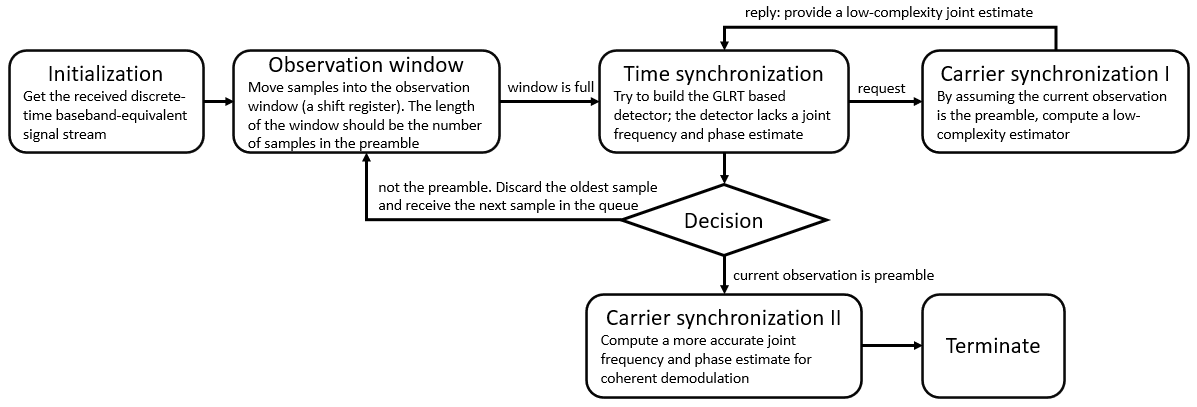
\includegraphics[width=6.5in]{signal_acquisition_chain.png}}
    \caption{Block diagram for analysis of the complete signal acquistion chain}
    \label{fig:sig_acquis_chain}
    \end{figure*}



